\section{La méthodologie}

La qualité du logiciel \FactDev{} est principalement dû à la rigueur dans l'application de la méthodologie de développement.

\subsection{Le respect de la méthode Scrum}
Au niveau de la gestion du développement par la méthode \Scrum{} nous avons tenu un \Backlog{} \ref{backlog}. Dans celui-ci se trouve l'ensemble des \UserStories{} et\TechnicalStories{} que nous avions à réaliser durant le projet. Ces \Stories{} ont été déterminée lors de \PlanningPoker durant les mêlées. C'est durant ces séances que nous déterminions le poids attribué à chacune des \Stories{} et comment les répartir sur les six \Sprints{} des deux \Releases.  

Lorsque nous ne pouvions nous voir pour assurer les mêlées quotidiennes, nous nous retrouvions sur une zone  de chat \textit{« \#irc »} que nous avions créé pour la circonstance. Ainsi, nous faisions le point sur l'évolution du projet et débattre sur des choix de conception.

Le \BurnUp{} ci-dessous montre l'assiduité et le respect de la méthode \Scrum{} durant le projet. 
\begin{figure}[H]
	\centering
	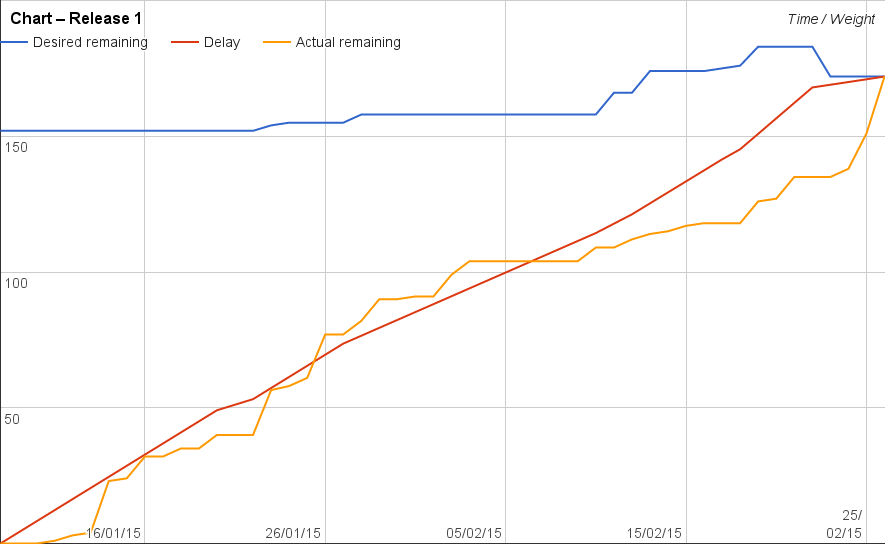
\includegraphics[width=0.7\linewidth]{screens/release1-chart.png}
	\caption{Burn Up chart de la première release}
	\label{fig:burnupchart-release1}
\end{figure}
La courbe rouge représente l'évolution théorique du projet durant les \Sprints{} de la première \Release. On constate que notre avancé (courbe orange)  suit globalement la courbe théorique. Cependant, l'on observe une baisse de notre activité durant la semaine du 5 février qui correspondait à notre période de vacance. De plus, on note également que lors du \Sprint{} 3 nous nous sommes trouvés en dessous de l'objectif. Cela s'explique par une augmentation du nombre de \Stories{} (courbe bleu) qui correspondait à des modifications ergonomiques où à la résolution de bugs. Néanmoins, nous sommes parvenus à finir nos \Sprints{} dans les temps. 

Chacun des \Sprints{} a été réalisé dans les temps et fut l'objet d'une démonstration auprès de M. \bsc{Migeon}. 

Dans l’ensemble la courbe suit bien la courbe théorique malgré une tendance en dessous du délai attendu. La coupure du milieu correspond à la semaine de vacances ou nous avons effectué une pause, sur la fin nous avons eu un retard à combler à cause de l’augmentation des stories liée aux bugs. Nous avons du transferérer quelques unes de ces dernières à la release d’après.


Une des manières la plus simple pour savoir si la méthodologie choisie correspondait bien aux résultats attendus et était bien adaptée est d'analyser les chiffres et les résultats que nous avons obtenus.

La méthode agile \Scrum{} que nous avons choisie nous a permis de bien répartir le travail en fonction de la disponibilité de chacun et de ses compétences techniques. En effet avec une moyenne de 10 \UserStories{} par \Sprint{} sur un total de 54, la durée des sprints (2 semaines) était bien adaptée à notre cycle de développement. Nous avons réalisé 6 sprints avec deux \Releases. Cette volonté de découper le travail par tranche de deux semaines était bénéfique dans le sens ou nous avons pu nous adapter aux attentes et aux évolutions des besoins du client. Nous reviendrons sur l'organisation plus bas avec le burnup chart.

Par ailleurs, la couverture des tests qui est aux alentours de 90\% sur la fin du projet nous a permis d'éviter un grand nombre de bugs ainsi que d'en trouver certains qui n'auraient pas forcément été détectés si il n'y avait pas eu de tests. Cependant les bugs par rapport à l'interface (clic sur un bouton qui provoque un plantage de l'application) n'ont pas pu être testé et nous avons du procéder à des tests manuels.

Enfin l'utilisation de \Github{} en étroite collaboration avec la méthode agile \Scrum{} a permis de pouvoir travailler depuis chez soit ce qui était indispensable dans ce contexte (nous ne pouvions programmer des mêlées tous les jours à cause des cours, etc). Le nombre de \PullRequest{} (95), issues (145), branches (91) et commits (1200) en est une preuve ainsi que la preuve de toute la communication que nous avons mis en place pour gérer ce projet.



